% Unofficial New York University Poster Template
% a fork of https://github.com/anishathalye/gemini
% also refer to https://github.com/k4rtik/uchicago-poster

% Adapted by Phillip Wang, all credits go to Tao Li


\documentclass[final]{beamer}

% ====================
% Packages
% ====================

\usepackage[T1]{fontenc}
 \usepackage[utf8]{luainputenc}
\usepackage{lmodern}
\usepackage[size=custom, width=120,height=72, scale=1]{beamerposter}
\usetheme{gemini}
\usecolortheme{cam}
\usepackage{graphicx}
\usepackage{booktabs}
\usepackage{tikz}
\usepackage{pgfplots}
\pgfplotsset{compat=1.14}
\usepackage{anyfontsize}

% ====================
% Lengths
% ====================

% If you have N columns, choose \sepwidth and \colwidth such that
% (N+1)*\sepwidth + N*\colwidth = \paperwidth
\newlength{\sepwidth}
\newlength{\colwidth}
\setlength{\sepwidth}{0.025\paperwidth}
\setlength{\colwidth}{0.3\paperwidth}

\newcommand{\separatorcolumn}{\begin{column}{\sepwidth}\end{column}}

% ====================
% Title
% ====================

\title{Long Short Term Memory}

\author{Prachi Ganpat Gore}

\institute[]{Department of Statistics, Kavayitri Bahinabai Chaudhari North Maharashtra University}

% ====================
% Footer (optional)
% ====================

\footercontent{
  \href{https://github.com/Prachi-Gore}{Github} \hfill
 \href{mailto:prachigore408@gmail.com}{prachigore408@gmail.com} \hfill
  \href{https://www.linkedin.com/in/prachi-gore-4772a11a5}{LinkedIn}}
% (can be left out to remove footer)

% ====================
% Logo (optional)
% ====================

% use this to include logos on the left and/or right side of the header:
% Left: institution
 % \logoleft{
\includegraphics[height=5cm]{logos/nyuad_white.png}}
% Right: funding agencies and other affilations 
%\logoright{\includegraphics[height=7cm]{logos/NSF.eps}}
% ====================
% Body
% ====================

\begin{document}



\begin{frame}[t]
\begin{columns}[t]
\separatorcolumn

\begin{column}{\colwidth}

  \begin{block}{Introduction}

    \begin{figure}
    \centering
    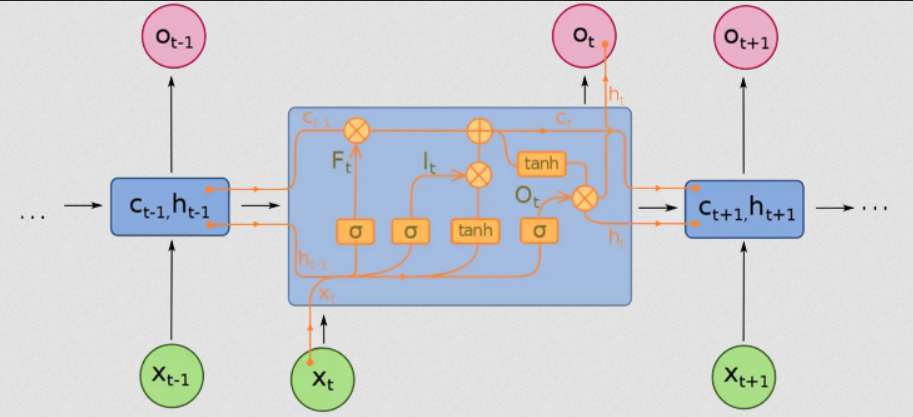
\includegraphics[width=0.7\textwidth]{intro.png}
    % \caption{ Medium.com}
    % \label{fig:example}
\end{figure}
LSTM has feedback connections, unlike conventional feed-forward neural networks. It can handle not only single data points (like photos) but also complete data streams (such as speech or video). LSTM can be used for tasks like unsegmented, linked handwriting recognition, or speech recognition.

   

   

  \end{block}

  \begin{block}{Structure of LSTM}

    The LSTM is made up of four neural networks and numerous memory blocks known as cells in a chain structure. A conventional LSTM unit consists of a cell, an input gate, an output gate, and a forget gate. The flow of information into and out of the cell is controlled by three gates, and the cell remembers values over arbitrary time intervals. The LSTM algorithm is well adapted to categorize, analyze, and predict time series of uncertain duration.

   \begin{figure}
    \centering
    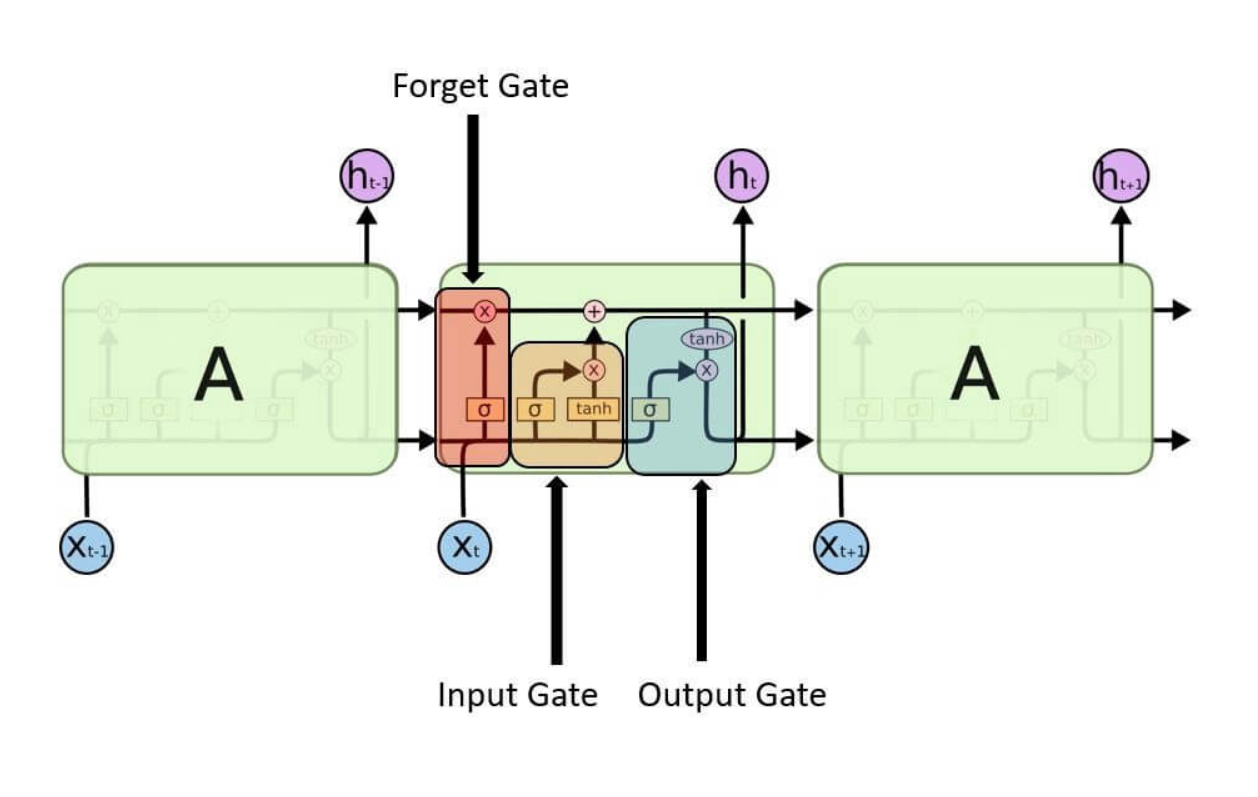
\includegraphics[ width=0.7\textwidth]{structure.png}   
\end{figure}

  \end{block}

  \begin{block}{Types of Gates}

    

    \begin{itemize}
      \item \textbf{Input Gate} It determines which of the input values should be used to change the memory.
      \item \textbf{Forget Gate} It finds the details that should be removed from the block.
      \item \textbf{Output Gate} The block’s input and memory are used to determine the output.
    \end{itemize}

    

  \end{block}

\end{column}

\separatorcolumn

\begin{column}{\colwidth}

  \begin{block}{LSTM Networks}
A sequence of repeating neural network modules makes up all recurrent neural networks. This repeating module in traditional RNNs will have a simple structure, such as a single tanh layer.\newline \\ 
 The output of the current time step becomes the input for the following time step, which is referred to as Recurrent. At each element of the sequence, the model examines not just the current input, but also what it knows about the prior ones.
\end{block}
\begin{block}{LSTM Cycle}
The LSTM cycle is divided into four steps:\newline
\begin{enumerate}[$\star$]
    
    \item  \space Using the forget gate, information to be forgotten is identified from a prior time step.\newline \newline
    \item \space Using input gate and tanh, new information is sought for updating cell state.\newline \newline
    \item \space The information from the two gates above is used to update the cell state.\newline \newline
    \item \space The output gate and the squashing operation provide useful information.

\end{enumerate}
\end{block} 
   

  
 \begin{block}{Bidirectional LSTMs}
Bidirectional LSTMs are an often discussed enhancement on LSTMs.

Each training sequence is presented forwards and backwards to two independent recurrent nets, both of which are coupled to the same output layer in Bidirectional Recurrent Neural Networks (BRNN). This means that the BRNN has comprehensive, sequential knowledge about all points before and after each point in a given sequence. There’s also no need to identify a (task-dependent) time window or goal delay size because the internet is free to use as much or as little of this context as it needs.\newline 



\begin{figure}
    \centering
    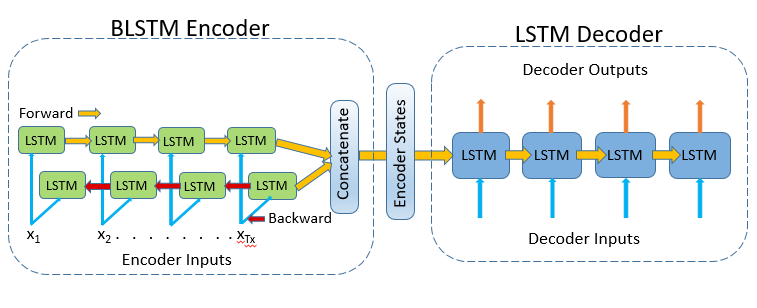
\includegraphics[ width=0.9\textwidth]{bidirectional.png}   
\end{figure}
\end{block} 

\end{column}

\separatorcolumn

\begin{column}{\colwidth}

  \begin{block}{Application}
   \begin{enumerate}
    \item  \hspace{0.2cm} Image captioning \newline 
    \item \hspace{0.2cm} space Machine translation \newline 
    \item \hspace{0.2cm} Language modelling \newline 
    \item \hspace{0.2cm} Handwriting generation \newline 
    \item \hspace{0.2cm} Question answering chatbots
\end{enumerate}
   
  \end{block}

  \begin{block}{Conclusion}

    \begin{enumerate}
    \item  \hspace{0.04cm} Long short-term memory (LSTM) is a deep learning architecture based on an artificial recurrent neural network (RNN).\newline
    \item  \hspace{0.04cm} LSTMs are a viable answer for problems involving sequences and time series.\newline
    \item  \hspace{0.04cm} The difficulty in training them is one of its disadvantages since even  a simple model takes a lot of time and system resources to train. However, this is only a hardware constraint.\newline
    \item  \hspace{0.04cm} The problem with traditional RNNs is that they can only use the prior contexts. BRNNs (Bidirectional RNNs) accomplish this by processing data in both directions.
    \end{enumerate}


    

  \end{block}

  \begin{block}{References}

    \nocite{*}
    \footnotesize{\bibliographystyle{plain}\bibliography{poster}}

  \end{block}

\end{column}

\separatorcolumn
\end{columns}
\end{frame}

\end{document}
